\chapter{Adronizzazione dei quark pesanti}

\section{Il Modello Standard (SM)}
\label{sec:SM}
    La fisica delle particelle elementari ha lo scopo di indagare la struttura microscopica della materia andando alla ricerca dei costituenti ultimi della realtà e delle loro interazioni. L'insieme delle teorie che meglio hanno saputo descrivere le evidenze sperimentali ha trovato una coerente formulazione teorica nel Modello Standard (Standard Model MS) della fisica delle particelle elementari. Ad oggi il modello prevede l'esistenza di tre tipologie di particelle elementari: quark, leptoni e bosoni mediatori i quali rappresentano tre delle quattro interazioni fondamentali, come rappresentato in figura~\ref{fig:1-standard-model}, esclusa quella gravitazionale non spiegabile con le teorie attuali.
    
    Il Modello Standard descrive dodici campi materiali dotati di massa che rappresentano i dodici sapori delle particelle materiali classificate in base alle loro interazioni. Queste particelle di spin \sfrac{1}{2} sono dette \textit{fermioni} poiché seguono la statistica di Fermi-Dirac. I fermioni si dividono in sei quark e sei leptoni: i primi sono soggetti a tutte le interazioni naturali, mentre i secondi non interagiscono con la forza forte \cite{CG_2007}.
    
    I \textit{quark} up e down, charm e strange, top e bottom sono organizzati in doppietti o generazioni nelle quali il primo elemento è generalmente il più massivo e ha carica elettrica positiva di modulo uguale a \sfrac{2}{3} quella dell'elettrone, mentre il secondo ha carica elettrica negativa modulo uguale a \sfrac{1}{3} di quella dell'elettrone.

    I \textit{leptoni} il cui nome deriva dal greco \textit{leptos}, leggero, poiché solitamente di massa inferiore ai quark, sono organizzati in doppietti: elettrone, muone e tauone e relativi neutrini elettronico, muonico e tauonico; i primi tre hanno carica elettrica negativa e unitaria, mentre i neutrini hanno carica elettrica e massa nulle secondo il Modello Standard. Le più recenti evidenze sperimentali mostrano però che i neutrini acquisiscono massa attraverso meccanismi ancora ignoti.

    Alle dodici particelle elementari corrispondono dodici \textit{antiparticelle} teorizzate per la prima volta nel 1929 dal fisico britannico Paul Dirac. Queste particelle hanno caratteristiche fisiche come massa, spin e vita media uguali a quelle delle relative particelle, ma numeri quantici e cariche opposte.

    \begin{figure}[t]
        \centering
        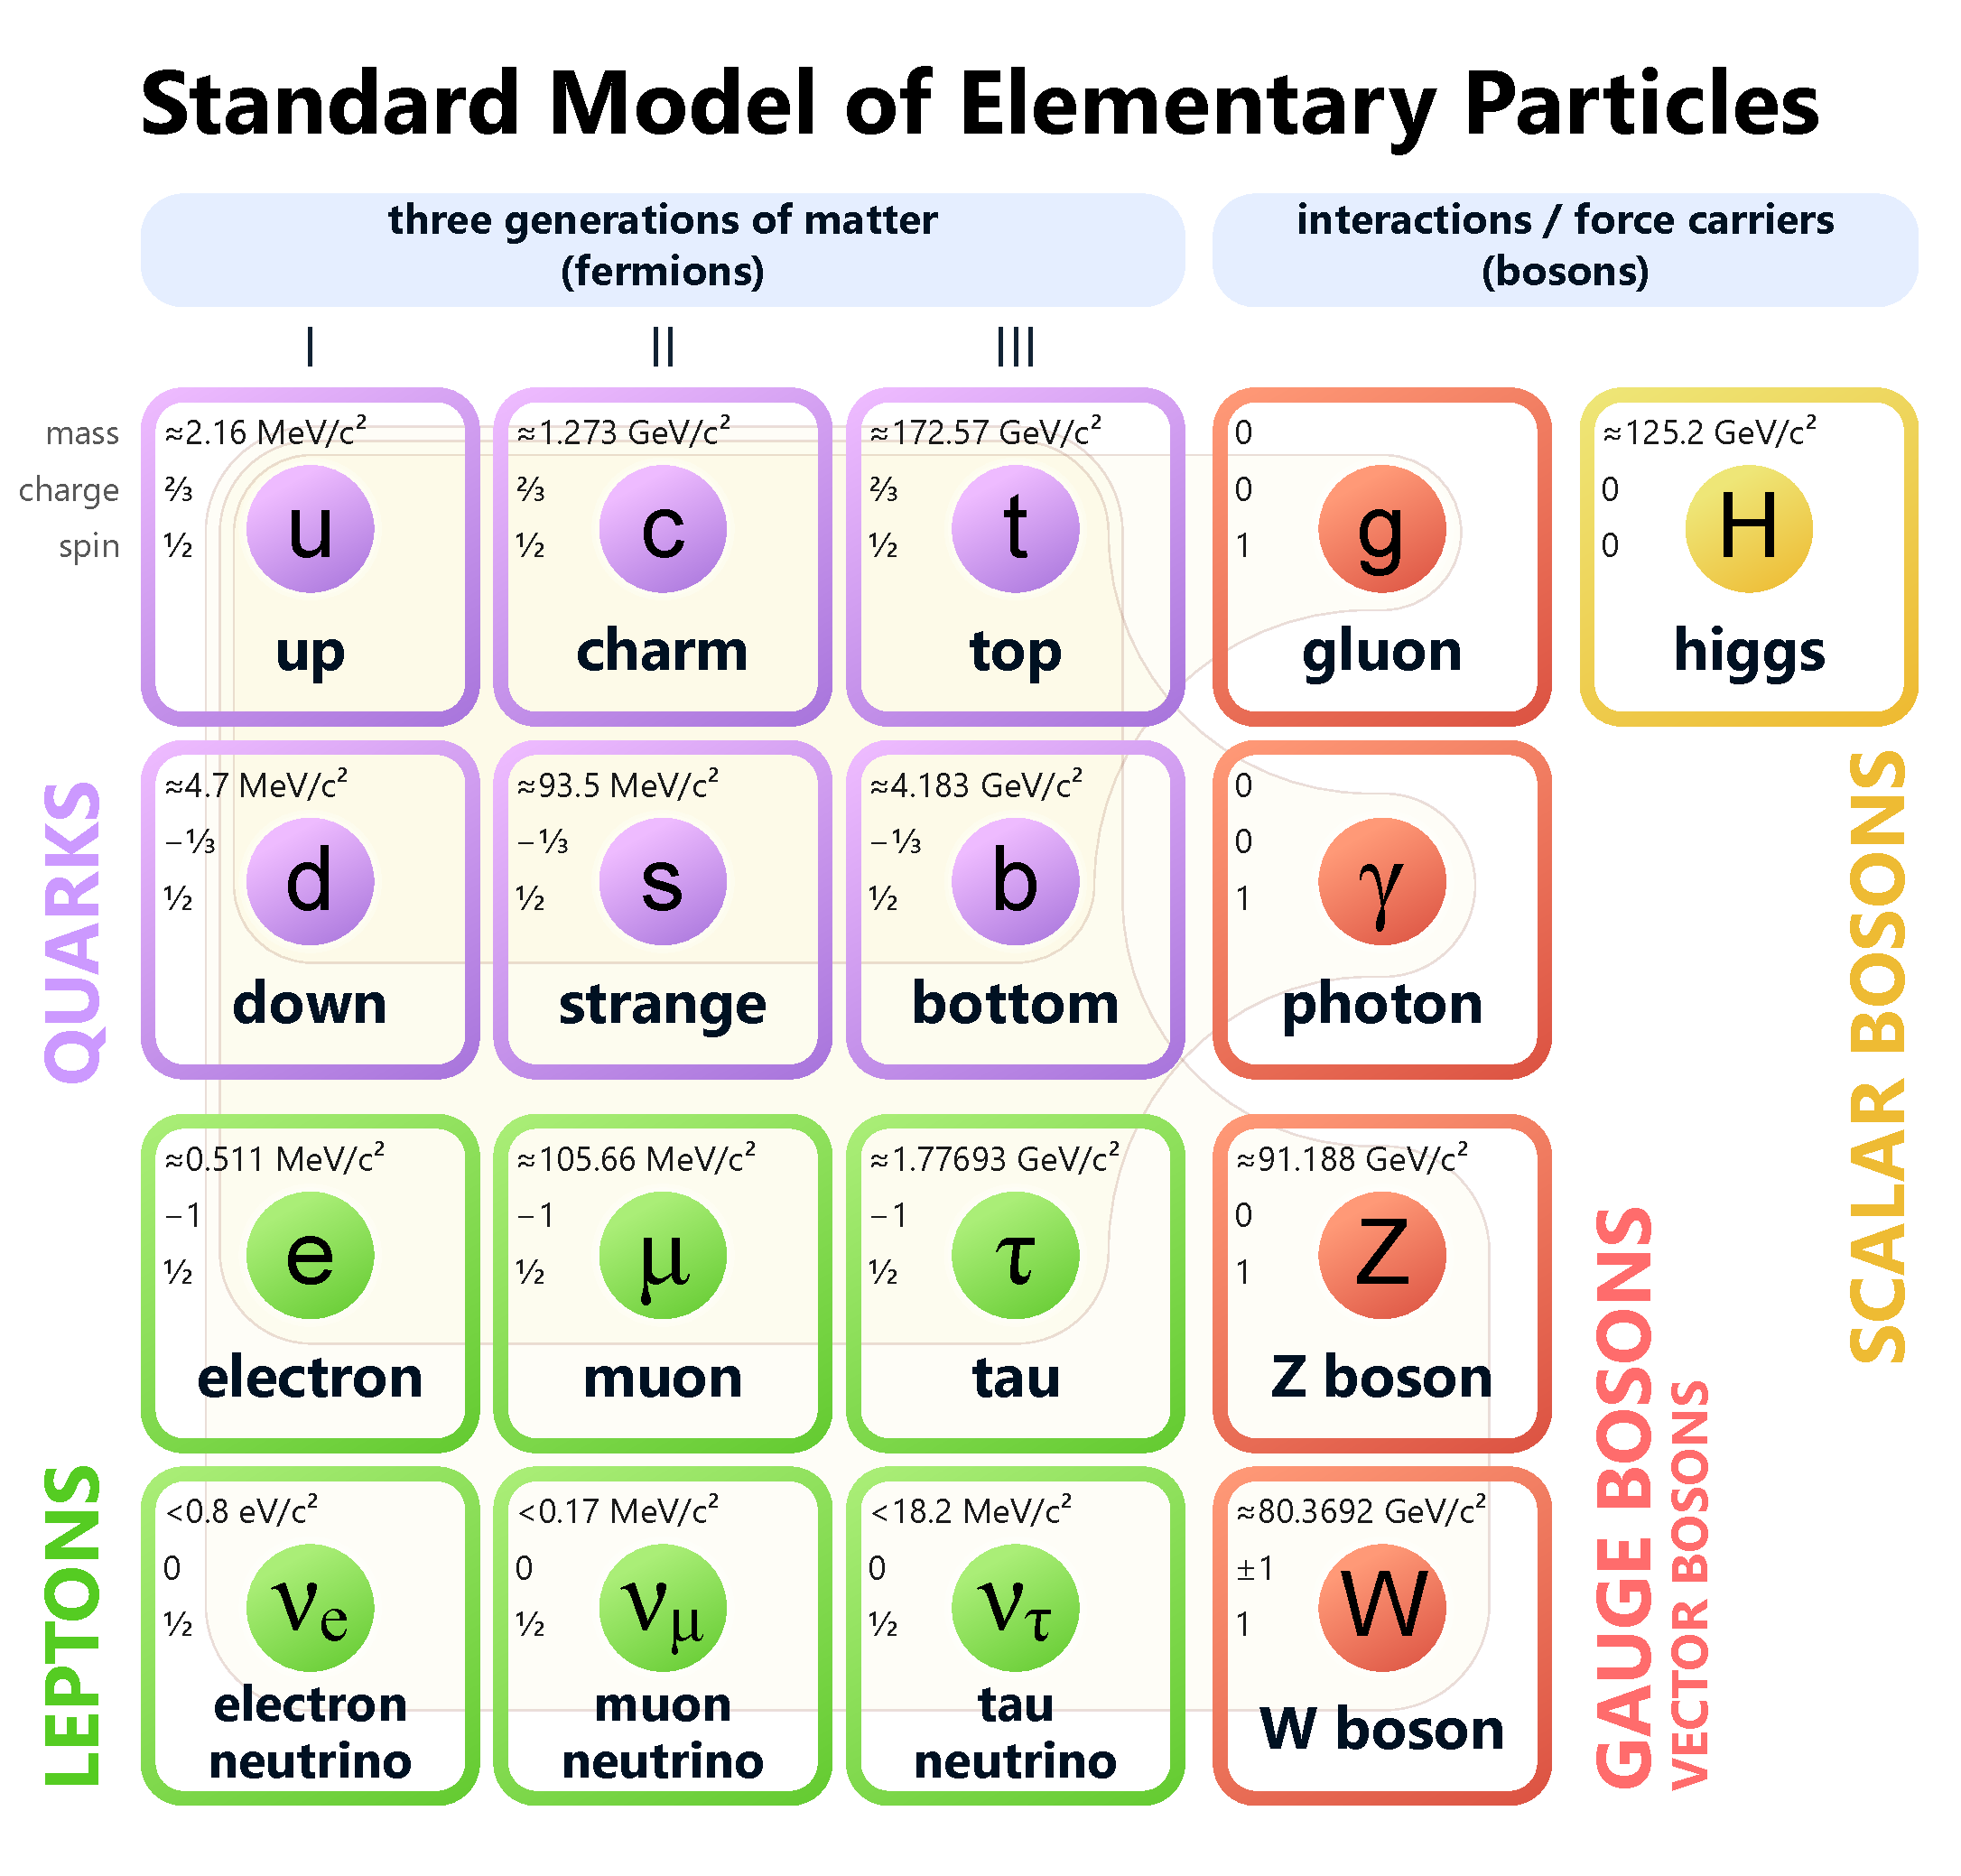
\includegraphics[width=0.8\linewidth]{res/fig/1-chapter/1-Standard_Model_of_Elementary_Particles}
        \caption{Schema delle particelle elementari presenti nel Modello Standard con relativa massa, carica e spin \cite{Wikimedia_Standard_Model}.}
        \label{fig:1-standard-model}
    \end{figure}

    In seguito troviamo le particelle mediatrici delle interazioni fondamentali. Queste particelle hanno spin 1 e sono dette \textit{bosoni}, vettore o di gauge, poiché seguono la statistica di Bose-Einstein e corrispondono alle tre interazioni fondamentali spiegate dal Modello Standard: otto gluoni $g$ mediatori dell'interazione forte, ciascuno con tre cariche di colore possibili, il fotone $\gamma$ mediatore dell'interazione elettromagnetica e i bosoni $Z^0$ e $W^\pm$ mediatori dell'interazione debole.

    Infine nel 2012 al CERN di Ginevra è stato scoperto dagli esperimenti ATLAS \cite{ATLAS_2012} e CMS \cite{CMS_2012} un bosone scalare di spin 0 chiamato bosone di Higgs $H$ associato al campo di Higgs col quale interagiscono tutte le particelle massive, fermioniche o bosoniche, per ottenere la loro massa tramite un meccanismo detto di \textit{rottura spontanea della simmetria} ipotizzato nel 1964 da F. Englert e R. Brout \cite{Englert_1964}, Peter W. Higgs \cite{Higgs_1964} e G. S. Guralnik, C. R. Hagen e T. W. B. Kibble \cite{GHK_1964}.
    
    È bene precisare che quelle presentate non sono particelle in senso classico, ma si fa sempre riferimento a campi quantizzati in cui i campi materiali possiedono cariche interne che permettono l'accoppiamento coi relativi campi di forza. Le teorie che compongono il Modello Standard sono teorie di campo quantizzato (Quantum Field Theory QFT): la \textit{Teoria Elettrodebole} che generalizza la Elettrodinamica Quantistica (Quantum Electrodynamics QED) e spiega i fenomeni elettromagnetici e di interazione debole e la \textit{Cromodinamica Quantistica} (Quantum Chromodynamics QCD) che spiega l'interazione tra quark attraverso lo scambio di gluoni. Ancora però non siamo capaci di descrivere in senso quantistico l'ultima interazione naturale, quella gravitazionale, per questo non presente nel modello.

    La fisica delle particelle studia fenomeni che coinvolgono corpi di dimensioni infinitesime a velocità prossime a quella della luce, è naturale quindi che il formalismo matematico del Modello Standard sia quello delle teorie di campo quantizzato che rappresentano l'evoluzione della meccanica quantistica in ambito relativistico, permettono lo studio di fenomeni sia quantistici sia relativistici e la creazione e distruzione di particelle.
    
    Il concetto di campo quantizzato è associato sia alle particelle sia alle loro interazioni: le prime sono interpretate come manifestazione del relativo campo, le ultime come scambio di quanti virtuali col campo di forza relativo all'interazione in gioco. Il Modello Standard è una teoria quantistica di campo di gauge locale che nel linguaggio della teoria dei gruppi di simmetrie si indica come $SU(3)_C \times SU(2)_L \times U(1)_Y$ in cui, da sinistra, sono racchiuse le tre interazioni naturali: forte, debole e elettromagnetica.

    Le interazioni nucleari forti sono a corto raggio per cui confinate all'interno dell'adrone e descritte dalla simmetria inviolata $SU(3)_C$, dove $C$ sta per colore, sulla quale poggia la \textit{Cromodinamica Quantistica} (QCD, vedi \ref{sec:QCD}). Lo spazio di $SU(3)_C$ ha $3^2 - 1 = 8$ generatori, cioè otto bosoni di gauge di spin 1 chiamati \textit{gluoni} $g$ mediatori dell'interazione forte. Come detto prima, tra i fermioni solo i quark sono soggetti all'interazione forte ovvero possiedono la carica, di colore, di $SU(3)_C$ che può assumere tre valori convenzionalmente indicati come $red\ (r)$, $green\ (g)$ e $blue\ (b)$ e rispettivi anticolori. I quark interagiscono tra loro scambiando gluoni dotati di una doppia carica di colore: colore-anticolore, a differenza dei fotoni che sono elettricamente neutri e cioè non possiedono la carica del campo che mediano. Per questo motivo i gluoni possono interagire tra loro, mentre i fotoni no. Matematicamente questa differenza è descritta dalla non abelianità del gruppo della QCD e dalla abelianità di quello della QED.

    Le interazioni debole e elettromagnetica sono descritte e unificate dalla simmetria $SU(2)_L \times U(1)_Y$, dove $L$ sta per leptoni e $Y$ per hypercharge, supercarica, e dal meccanismo di Higgs di rottura della simmetria che permette alle particelle di acquisire la loro massa. Nella forma più semplice questo meccanismo produce 4 bosoni di gauge, vettori, di spin 1: due neutri di cui uno massivo ($Z^0$) e uno privo di massa ($\gamma$) e due carichi e massivi ($W^\pm$) più un bosone scalare di spin 0, il bosone di Higgs ($H$) \cite{Vitale_1995}.

    \newpage

\section{Adroni e Modello a Quark (QPM)}
\label{sec:QPM}
    I dati relativi agli esperimenti di diffusione profondamente inelastica e-p suggerirono un modello fenomenologico dell'interno dell'adrone che prese il nome di \textit{modello a partoni}. Proposto da Richard Feynman nel 1969, questo modello ipotizza che i nucleoni, costituenti del nucleo atomico, non siano particelle elementari, ma siano costituiti da centri diffusori puntiformi detti partoni. In seguito i partoni vennero identificati con quark e gluoni e oggigiorno il termine \textit{partone} indica quark e gluoni costituenti di un adrone indifferentemente.
    
    Col termine \textit{adrone} indichiamo le particelle composte di quark, solitamente più pesanti dei leptoni, il cui nome deriva dal greco \textit{hadrón}, pesante, che possiedono carica di colore e che possono quindi interagire tramite forza forte. Solitamente i quark che costituiscono l'adrone vengono chiamati \textit{quark di valenza}, mentre gluoni, quark e antiquark virtuali generati dalle forze forti che uniscono i quark di valenza vengono chiamati \textit{mare}.

    Il Modello a Quark noto anche come Modello a Partoni o Modello Quark-Partone (Quark-Parton Model QPM), è un modello che descrive gli adroni come composti di quark fornendone una semplice classificazione. Poiché i quark liberi, ovvero non legati assieme all'interno di un adrone, non sono mai stati osservati, è stato postulato che i quark siano confinati all'interno degli adroni come verrà chiarito meglio in \ref{sec:QCD}.

\section{La Cromodinamica Quantistica (QCD)}
\label{sec:QCD}
    Chiarita la struttura interna degli adroni, la QCD ci fornirà ora un quadro teorico più completo per descrivere le interazioni tra quark e gluoni.

    Come già accennato in \ref{sec:SM}, la \textit{Cromodinamica Quantistica} (QCD) è la teoria di campo quantizzato che descrive l'interazione forte attraverso scambi di gluoni. È una teoria di gauge non abeliana con gruppo di simmetria $SU(3)_C$, possiede quindi 8 generatori o bosoni di gauge vettori di spin 1 mediatori dell'interazione forte, chiamati \textit{gluoni} $g$ che possiedono a loro volta una doppia carica di colore: colore-anticolore. La QCD mostra come le uniche combinazioni di quark possibili per formare un adrone siano \textit{mesoni} (coppie quark-antiquark) e \textit{barioni} (tripletti di quark e antiquark). Nonostante questo sono stati sperimentalmente osservati stati esotici di quattro e cinque quark e stati legati di soli gluoni.

    Sperimentalmente non sono mai stati osservati quark liberi a causa del cosiddetto \textit{confinamento di colore}: i quark si legano in doppietti o tripletti che devono necessariamente essere di colore bianco ovvero neutri cioè con carica di colore nulla. Il confinamento di colore prevede infatti che sia energeticamente favorevole la produzione di una ulteriore coppia quark-antiquark, chiamata \textit{jet adronico}, nel caso si tentasse la separazione tra quark e antiquark in un mesone fornendo energia, rendendo impossibile l'ottenimento di un quark libero come mostrato in figura~\ref{fig:2-hadron-jet}.

    \begin{figure}[t]
        \centering
        \includesvg[width=0.75\linewidth]{1-chapter/2-Quark_confinement}
        \caption{Rappresentazione grafica della rottura di stringa QCD nel vuoto. La figura mostra come venga generata una coppia quark-antiquark quando un mesone riceve energia sufficiente: il gluone che lega i due quark si "allunga" finché non si spezza e forma una nuova coppia quark-antiquark \cite{Wikimedia_Quark_Confinement}.}
        \label{fig:2-hadron-jet}
    \end{figure}

    Un'altra importante proprietà della QCD è la \textit{libertà asintotica} secondo la quale l'intensità dell'interazione forte è estremamente alta a basse scale di energia o grandi distanze. Questo contribuisce alla stabilità dello stato legato dei quark negli adroni e sfavorisce l'esistenza di quark liberi. In regime di alte energie o piccole distanze invece l'interazione è molto meno intensa permettendo l'utilizzo di approcci di calcolo \textit{perturbativi} \cite{BGS_2012}.

    \subsection{Cromodinamica Quantistica Perturbativa (pQCD)}
        Due sono gli approcci tradizionali alla QCD perturbativa. Il primo è il metodo detto dell'\textit{Elemento di Matrice} (Matrix Element ME) \cite{Vitale_1995} in cui i diagrammi di Feynman sono calcolati compiutamente per ogni ordine. In linea di principio questo metodo è il più rigoroso, ma incontra grandi difficoltà già al terzo ordine, tanto che i soli calcoli ad ora disponibili si arrestano al secondo ordine perturbativo.

        Il secondo approccio è quello della Cascata di Partoni (\textit{Parton Shower} PS) \cite{Bambah_199224}. Si tratta in questo caso di produrre un numero arbitrario di partoni che combinati tra loro generano gli eventi a più jet. Questo è possibile poiché non vengono utilizzate le espressioni complete degli elementi di matrice, ma solo delle loro approssimazioni.

        Per determinare il regime in cui la teoria perturbativa è applicabile è necessario valutare il valore di $Q^2 = - q^2$ con $q$ \textit{quadrimomento} trasferito nella collisione e segno negativo derivante dalla metrica di Minkowski \cite{Altarelli_2004}. Nel nostro caso, per grandi valori di $Q^2$, l'interazione forte diventa meno intensa e può quindi essere trattata con metodi perturbativi rendendo così la \textit{QCD perturbativa} (perturbative QCD, pQCD) un approccio valido.

\newpage

\section{Plasma di Quark e Gluoni (QGP)}
    Un modello euristico che permette di descrivere i quark confinati negli adroni è il \textit{MIT bang model} \cite{Wong_1994}. Secondo questo modello i quark sono particelle di massa nulla all'interno di una scatola di dimensioni finite e infinitamente massivi all'esterno. In questo modo il confinamento non è altro che il risultato del bilancio tra pressione esterna e interna, quest'ultima data dall'energia cinetica dei quark stessi. I gluoni scambiati tra quark sono anch'essi confinati nella scatola la cui carica di colore totale deve essere nulla.
    
    Questo modello fornisce ragioni sufficienti del perché ci aspettiamo di trovare nuove fasi della materia formata da quark oltre alla materia adronica: se la pressione esercitata dai quark interni crescesse oltre il valore della pressione esterna si verrebbe a creare un nuovo stato della materia a temperature e pressioni altissime in cui quark e gluoni non sono più legati, chiamato \textit{Plasma di Quark e Gluoni} (Quark Gluon Plasma QGP). Una rappresentazione indicativa del diagramma di fase della materia fortemente interagente è riportato in figura~\ref{fig:3-phase-diag-qgp}.
    
    \begin{figure}[h]
        \centering
        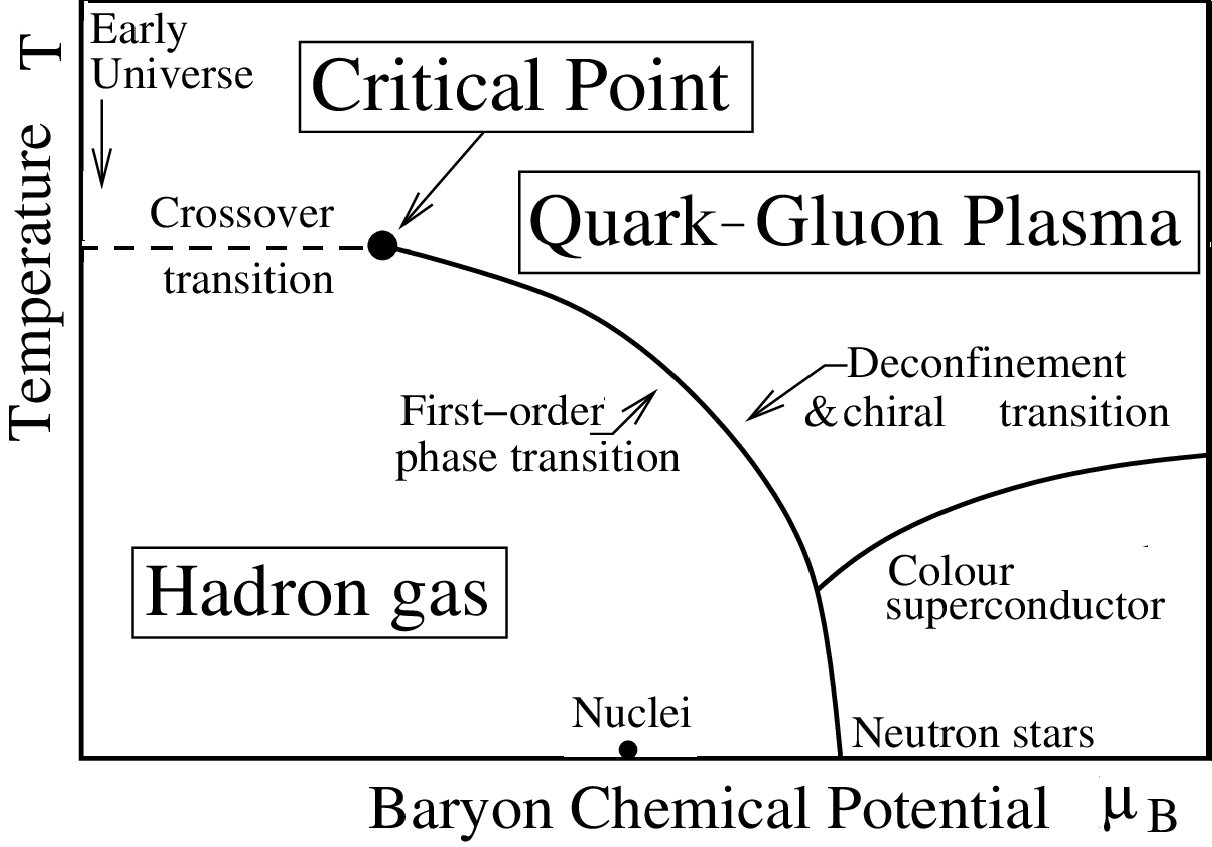
\includegraphics[width=0.7\linewidth]{res/fig/1-chapter/3-PhasDiagQGP.png}
        \caption{Diagramma di fase qualitativo della materia fortemente interagente \cite{Wikipedia_PhasDiagQGP}.}
        \label{fig:3-phase-diag-qgp}
    \end{figure}
    
    Quando il sistema raggiunge la temperatura critica $T_C \approx$ \qtyrange[range-phrase = --, range-units = single]{150}{200}{\mega \eV} avviene una transizione di fase del primo ordine tra materia adronica e QGP. La densità di energia nell'intorno di questa transizione presenta una discontinuità detta \textit{calore latente di deconfinamento}. La regione di basse temperature e alte densità è detta regione di \textit{diquark matter} o regione di \textit{superconduttività di calore}. In queste condizioni avviene la formazione di coppie di quark non neutre di colore analoghe alle coppie di Cooper dei superconduttori.

    La capacità dei barioni di ricombinare i quark per formare nuovi adroni è chiamata potenziale chimico barionico o \textit{potenziale bariochimico}, influenza la composizione di barioni e mesoni prodotti nelle collisioni ed è formulato come segue:
    
    \begin{equation}
        \mu_B = \dv{E}{N_B}.
    \end{equation}

    Un caso particolare è il QGP fortemente legato (\textit{strongly-coupled QGP} sQGP) nel quale le interazioni tra quark e gluoni sono estremamente forti e non possono essere trattate con gli approcci convenzionali basati sulla teoria perturbativa.

\section{Collisioni tra particelle}
\label{sec:COLLISION}
Nello studio della QCD le predizioni teoriche si basano sul calcolo perturbativo di sistemi di quark e gluoni dotati di colore, carica che rappresenta i gradi di libertà a piccola distanza, le osservazioni sperimentali invece sono fatte su stati finali di adroni, ovvero stati legati di partoni in singoletto di colore. È quindi necessario analizzare i processi che portano allo stato finale cercando di descriverli con le caratteristiche dell'interazione partonica iniziale.

Le collisioni tra ioni pesanti (A-A) accelerati ad energie relativistiche sono lo strumento migliore per studiare la materia nucleare in condizioni estreme di temperatura e densità di energia. È così possibile produrre numerose collisioni simultanee tra i vari nucleoni presenti nei due nuclei collidenti creando un sistema ad altissima densità di partoni prodotti interagenti tra loro e permettono di riprodurre in laboratorio le condizioni dell'universo primordiale frazioni di secondo dopo il Big-Bang, come il QGP.

L'avvenuta formazione di uno stato di QGP può essere verificata attraverso la misura di diversi effetti come gli spettri di impulso delle particelle prodotte, la soppressione o l'aumento di produzione di stati legati di quark pesanti e la presenza di moti collettivi. È poi necessario confrontare le misure ottenute con quelle di scontri p-p alle stesse energie per assicurarsi che lo stato prodotto in collisioni A-A non sia una semplice sovrapposizione di scontri p-p e che si tratti effettivamente di QGP e non di un gas di adroni eccezionalmente denso.

A complicare ulteriormente questo quadro, le differenze tra i risultati ottenuti in collisioni A-A e p-p potrebbero essere dovute all'utilizzo di proiettili estesi, i nuclei, nel primo caso, in particolare per le modifiche alle funzioni di distribuzione partonica nei nucleoni appartenenti ad un nucleo e alla presenza di scattering multipli prima di un hard scattering. È quindi necessario accertarsi che i risultati ottenuti in collisioni A-A non dipendano da questi effetti denominati di \textit{effetti di stato iniziale}. Per fare ciò vengono utilizzate collisioni protone-ione p-A.

Negli anni sono state ottenute numerose evidenze sperimentali a favore della formazione del QGP in collisioni A-A da esperimenti ai collider SPS~\cite{NA60_2021}, RHIC e LHC~\cite{ALICE_2024}. Recentemente però in collisioni p-p e p-A sono stati \textit{osservati} gli stessi effetti normalmente associati al deconfinamento di quark, ovvero al QGP, e per questo motivo assolutamente non attesi: aumento di produzione di particelle strange, evidenze di collettività a basso impulso trasverso e presenza di correlazioni a lungo raggio con conseguenti misure di flusso ellittico e armoniche superiori. L'esperimento ALICE in particolare ha osservato un aumento della stranezza, ovvero della produzione di particelle contenenti al loro interno uno o più quark strange $s$, in funzione della molteplicità dell'evento \cite{ALICE_2008} confrontando collisioni p-p, p-A e A-A in cui eventi p-p ad alta molteplicità mostrano risultati molto simili a quelli ottenuti in collisioni A-A \cite{RHIC_2020} \cite{ALICE_pp_2017} \cite{ALICE_pp_pPb_pBPb_2024}. Una possibile spiegazione di questo fenomeno consiste nell'assumere che anche in collisioni p-p ad alta molteplicità, in cui cioè avvenga più di una collisione partone-partone tra i costituenti dei due protoni interagenti, si possa creare uno stato di QGP. Questa ipotesi può spiegare la presenza di effetti collettivi negli stati finali. D'altro canto, le ridotte dimensioni del QGP eventualmente creato in collisioni p-p e p-A sarebbero in accordo con la \textit{mancata osservazione} di fenomeni di perdita di energia per partoni ad alto impulso trasverso nell'attraversare un mezzo con elevata densità di partoni liberi.

    \subsection{Collisioni tra ioni pesanti}
        L'unico metodo conosciuto per creare condizioni di temperatura e densità energetica così elevate da produrre artificialmente il QGP sono le collisioni tra ioni pesanti ultrarelativistici, $\beta = v/c \approx 1$.

        Le dimensioni dei nuclei degli ioni collidenti sono molto maggiori rispetto a tutte le scale proprie della fisica delle particelle elementari che appunto studia i quark costituenti dei nucleoni che a loro volta costituiscono il nucleo. Per questa ragione la \textit{geometria delle collisioni} gioca un ruolo fondamentale nell'analisi e interpretazione dei risultati sperimentali.

        Nel sistema del centro di massa, grazie alla contrazione di Lorentz nella direzione longitudinale di propagazione del fascio, i due nuclei possono essere visti nel piano trasverso come dischi sottili di raggio $2 R_A \approx 2 A^{\frac{1}{3}}$ con $A$ numero di nucleoni. Una rappresentazione grafica del processo è rappresentata in figura~\ref{fig:4-centrality}, alcune delle quantità rilevanti sono~\cite{Salgado_2009}:
        \begin{description}
            \item[\textit{parametro di impatto} $b$] distanza tra gli assi centrali dei nuclei in procinto di collidere, che caratterizza la centralità della collisione: l'urto si dirà centrale se $b$ è molto piccolo e lo scontro è pressoché frontale, si dirà invece periferico se $b$ è grande rispetto alle dimensioni delle particelle. La centralità dell'evento si esprime tipicamente in percentuali di sezione d'urto totale.
            
            \item[numero di nucleoni coinvolti] i \textit{participants}, $N_{part}$ all'interno dei nuclei collidenti ossia il numero di neutroni e protoni dei due ioni che prendono parte alla collisione. I restanti vengono chiamati spettatori, \textit{spectators}, e proseguono nella loro traiettoria quasi imperturbati. 
            
            \item[numero totale di collisioni nucleone-nucleone incoerenti] $N_{coll}$.
        \end{description}
        Numerosi modelli teorici sono stati sviluppati per descrivere le dinamiche di collisione a partire da queste quantità.

        \begin{figure}[t]
            \centering
            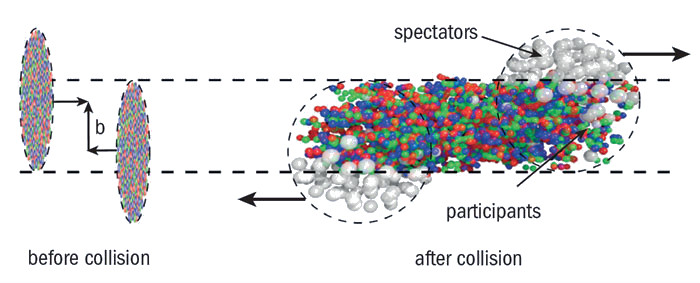
\includegraphics[width=0.8\linewidth]{res/fig/1-chapter/4-centrality.png}
            \caption{Rappresentazione geometrica della collisione tra i nuclei di due ioni pesanti~\cite{Toia_2013}. Come mostrato, la collisione può coinvolgere solamente parte dei nucleoni presenti (\textit{participants}), lasciandone fuori altri (\textit{spectators}).}
            \label{fig:4-centrality}
        \end{figure}

         In fisica subnucleare si è soliti descrivere le traiettorie delle particelle in termini della variabile \textit{rapidità} $y$ o della variabile \textit{pseudorapidità} $\eta$, definite rispettivamente come:
         \begin{equation*}
             y = \frac{1}{2} \ln(\frac{E + p_L}{E - p_L})
         \end{equation*}
        con $E = \sqrt{p^2 c^2 + m^2 c^4}$ energia relativistica e $p_L$ componente longitudinale del momento della particella rispetto all'asse del fascio e:
        \begin{equation*}
            \eta = \frac{1}{2} \ln(\frac{p + p_L}{p - p_L}) = - \ln(\tan{\frac{\theta}{2}})
        \end{equation*}
        con $\theta$ angolo tra impulso della particella e asse del fascio. Per particelle di massa nulla come il fotone rapidità e pseudorapidità coincidono, mentre per particelle massive questa corrispondenza vale solo nel limite ultrarelativistico.

\section{Evoluzione del QGP}
    Avvenuta la collisione si ha la formazione di un plasma di quark e gluoni solo nel caso in cui vengano raggiunte le condizioni critiche di temperatura e densità di energia~\cite{Andronic_2014}.
    
    Nel caso in cui le condizioni richieste non venissero raggiunte il sistema entrerebbe in \textit{evoluzione idrodinamica}, figura~\ref{fig:5-time-evol-qgp} a) a sinistra. Questo è il caso tipico delle collisioni tra protoni p-p o di collisioni tra ioni pesanti A-A non sufficientemente energetiche e centrali. Subito dopo la collisione vi è una breve fase \textit{pre-adronica}, in grigio, in cui i quark prodotti adronizzano in un "vuoto" QCD dopo la quale il sistema evolve come \textit{gas di adroni}, in sostanza attraverso processi di frammentazione. Sebbene avvenga un sostanziale incremento di pressione e temperatura non si manifesta alcun deconfinamento di partoni in questo caso.

    Nel caso in cui invece la collisione fosse sufficientemente energetica da soddisfare le condizioni di creazione del QGP, il processo rappresentato in figura~\ref{fig:5-time-evol-qgp} b) a destra è più complesso~\cite{Strazzi_2019}:
    \begin{enumerate}
        \item \textit{Pre-Equilibrium phase} ($t < \tau_0 \approx$ \qty[per-mode = symbol]{1}{\femto \meter \per \clight}): in questa fase i partoni diffondono l'uno sull'altro producendo quark e gluoni deconfinati in abbondanza. Vengono prodotte molte particelle ad elevato impulso trasverso ($p_T \gg$ \qty[per-mode = symbol]{1}{\giga \eV \per \clight}) e una grande quantità di fotoni sia reali sia virtuali che decadono in coppie leptone-antileptone.

        \item \textit{Termalizzazione} ($t \approx$ \qtyrange[range-phrase = --, range-units = single, per-mode = symbol]{1}{10}{\femto \meter \per \clight}): questa fase è caratterizzata dalle interazioni elastiche e inelastiche tra i partoni del QGP. Le interazioni inelastiche hanno la peculiarità di poter cambiare la composizione di sapore delle particelle. A causa della pressione interna il sistema all'equilibrio termico inizia ad espandersi rapidamente raffreddandosi di conseguenza e convertendosi in un gas adronico (\textit{fase mista}).

        \item \textit{Adronizzazione} ($t \approx$ \qty[per-mode = symbol]{20}{\femto \meter \per \clight}): durante l'espansione il sistema si raffredda raggiungendo il valore critico di densità che dà inizio al processo di adronizzazione in cui quark e gluoni del QGP condensano in nuovi adroni. L'interazione tra gli adroni continua finché il relativo tasso è in grado di sostenere l'espansione del QGP e raggiunto un certo valore della temperatura cessano le interazione inelastiche tra i costituenti del sistema. Dopodiché la composizione di sapore del QGP si fissa raggiungendo il congelamento chimico (\textit{chemical freeze-out}).

        \item \textit{Congelamento termico} (\textit{thermal freeze-out}): quando la densità del sistema è tale da rendere la distanza media tra gli adroni maggiore del raggio di azione dell'interazione forte, per $T_{fo} \approx$ \qty{120}{\mega \eV}, le diffusioni elastiche tra gli adroni cessano e resta fisso anche lo spettro cinematico della materia risultante.
    \end{enumerate}

    \begin{figure}[h]
        \centering
        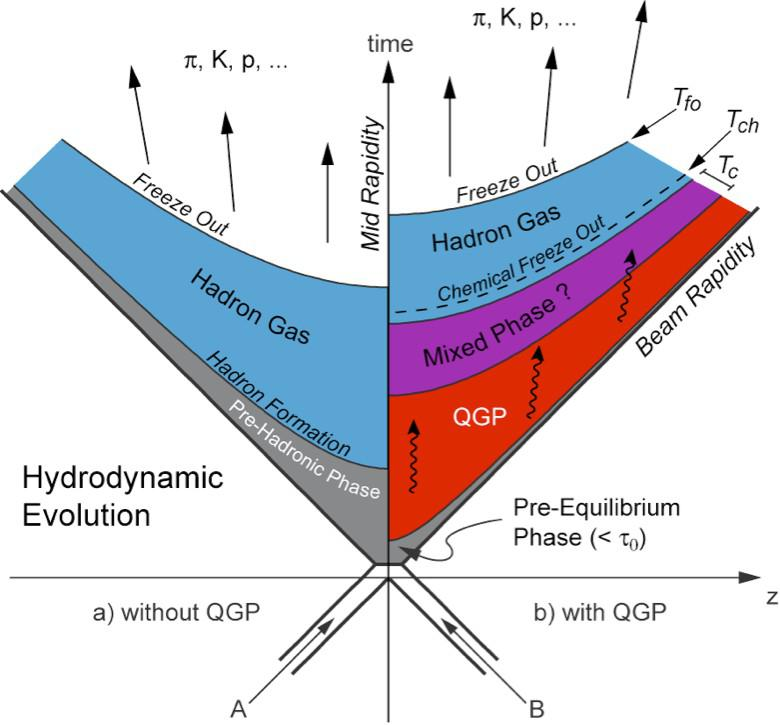
\includegraphics[width=0.65\linewidth]{res/fig/1-chapter/5-TimeEvolQGP.jpg}
        \caption{Evoluzione temporale di una collisione tra ioni pesanti in un piano simile a quello di Minkowski. a) a sinistra il caso in cui il sistema entra in evoluzione idrodinamica e diventa un gas adronico senza formazione di QGP. b) a destra il caso in cui le condizioni permettono la formazione del QGP che perdendo energia si trasforma anch'esso in gas adronico~\cite{ES_2011}.}
        \label{fig:5-time-evol-qgp}
    \end{figure}

\section{Adronizzazione di sapori pesanti in collisioni p-p}
    Nello studio delle proprietà del QGP i quark pesanti charm $c$ e bottom $b$ rivestono un ruolo fondamentale poiché in virtù della loro massa elevata vengono prodotti in collisioni \textit{hard}, ossia ad alto momento $Q^2$ trasferito, tra i partoni dei nucleoni nelle primissime fasi della collisione nucleo-nucleo, prima ancora che il sistema termalizzi e si formi lo stato di QGP. Questi quark quindi si propagano attraverso il sistema ultra-denso interagendo coi suoi costituenti e fornendo una \textit{misura diretta delle sue proprietà}. Per poter comprendere appieno una misura effettuata in collisioni A-A però è necessario confrontarla con la stessa misura effettuata in collisioni p-p e p-A, come chiarito in~\ref{sec:COLLISION}.

    L'adronizzazione di sapori pesanti in collisioni p-p attraverso il processo di \textit{frammentazione} viene descritta matematicamente attraverso il \textit{teorema di fattorizzazione}~\cite{CSS_2004}. Data la scala del momento $Q^2$ trasferito nel processo di collisione, esso consiste nel separare il contributo perturbativo ad alta energia della produzione del \textit{leading parton} dalla successiva conversione nello stato adronico a bassa energia non perturbativo. Il processo complessivo è:
    \begin{equation*}
        p + p \to h + X
    \end{equation*}
    dove l'adrone di riferimento $h$ è dato dal decadimento del partone $c$ proveniente dallo scattering $a + b$ dei partoni del protone $a + b \to c + d$.

    Possiamo ora esprimere la sezione d'urto invariante della produzione dell'adrone nel medio range di rapidità per collisioni p-p come:
    \begin{equation*}
        \dv{\sigma_{pp}^h}{y d^2 p_T} = K \sum_{abcd}{ \int{ \dd{x_a} \dd{x_b} f_{a}(x_a,Q^2) f_{b}(x_b,Q^2) \dv{\hat{t}} \sigma(a + b \to c + d) \frac{D_{{h}/{c}}^0}{\pi z_c}}}
    \end{equation*}
    con:
    \begin{description}
        \item[$f_i(x_i,Q^2)$] \textit{Funzioni di Distribuzione dei Partoni} (PDF) riferite ai partoni del protone.

        \item[$\dv{\hat{t}} \sigma(a + b \to c + d)$] sezione d'urto elementare perturbativa QCD della produzione della particella $c$ a partire dallo scattering dei partoni $a + b$.

        \item[$D_{{h}/{c}}^0$] \textit{Funzione di Frammentazione} (FF): elemento adimensionale che fornisce la probabilità che il partone $c$ adronizzi nell'adrone finale $h$ emettendo gluoni e trasportando una frazione del momento del partone iniziale. Le FF non sono calcolabili perturbativamente e devono essere quindi misurate sperimentalmente.
    \end{description}

    \subsection{Funzioni di Distribuzione di Partoni (PDF)}
        Le evidenze sperimentali hanno mostrato che gli adroni non sono particelle elementari puntiformi, ma sono composte da \textit{partoni}: quark e gluoni. Come detto in~\ref{sec:QPM}, i costituenti interni di un adrone possono essere divisi in \textit{quark di valenza}, ossia i quark che effettivamente determinano i numeri quantici dell'adrone come $uud$ per il protone p, e in partoni del mare o \textit{mare}, ossia tutti i restanti partoni, gluoni e quark, creati e distrutti nei processi virtuali che avvengono all'interno dell'adrone secondo la QCD.

        Consideriamo l'esempio del protone p. Denotiamo con
        \begin{description}
            \item[$q^v(x)$] la densità di probabilità di un quark di valenza,

            \item[$q^s(x)$] la densità di probabilità di un quark del mare,

            \item[$g(x)$] la densità di probabilità di un gluone,

            \item[$x$] la frazione del momento totale trasportato da un quark $q$ o un gluone $g$.
        \end{description}
        Sapendo che i quark di valenza del protone sono $uud$, otteniamo la condizione:
        \begin{equation*}
            \int_{0}^{1}{\dd{x} u^v(x)} = 2 \qquad \int_{0}^{1}{\dd{x} d^v(x)} = 1.
        \end{equation*}
        I quark del mare sono sempre prodotti in coppie $q\bar{q}$ e danno un contributo nullo al numero barionico:
        \begin{equation*}
            \int_{0}^{1}{\dd{x} [u^s(x) - \bar{u}^s(x)]} = 0 \qquad \int_{0}^{1}{\dd{x} [d^s(x) - \bar{d}^s(x)]} = 0.
        \end{equation*}
        La stessa condizione è valida per gli altri quark del mare $s^s$, $c^s$, $b^s$ e $t^s$.
        Il momento totale portato da tutti i partoni deve contribuire al momento totale, perciò si ha la condizione:
        \begin{equation*}
            \int_{0}^{1}{\dd{x} x [u^{v}(x) + d^{v}(x) + \sum_{q} (q^{s}(x) + \bar{q}^{s}(x))]} = 1
        \end{equation*}
        I quark pesanti sono inclusi nella presente trattazione, ma sono attivi solamente se la scala di energia $Q$ del sistema è superiore alla massa $m_q$ del quark pesante stesso.

        In figura \ref{fig:6-pdf-momentum-proton} sono mostrate le funzioni di distribuzione del momento dei partoni del protone a $Q^2 =$ \qty{10}{\giga \eV^2}. È interessante notare come il termine dei gluoni rappresenti circa metà del momento totale.

        \begin{figure}[h]
            \centering
            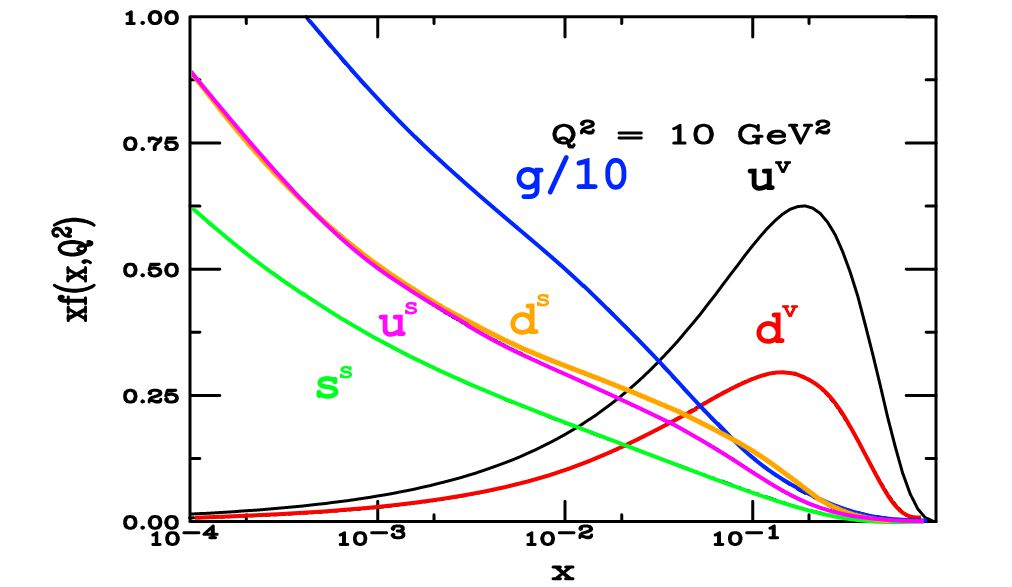
\includegraphics[width=0.71\linewidth]{res/fig/1-chapter/6-pdf-momentum-proton.jpg}
            \caption{Funzioni di distribuzione del momento dei partoni del protone $xf(x)$, secondo la parametrizzazione CTEQ6M dei partoni a $Q^2 =$ \qty{10}{\giga \eV^2}. La distribuzione dei gluoni è divisa per 10 per migliorarne la visualizzazione \ref{fig:6-pdf-momentum-proton}.}
            \label{fig:6-pdf-momentum-proton}
        \end{figure}

\newpage

    \subsection{Funzioni di Frammentazione (FF)}
        Per comprendere meglio le Funzioni di Frammentazione consideriamo il processo di annichilazione di un sistema elettrone-positrone per produrre una coppia quark-antiquark~\cite{Vogt_2007}
        \begin{equation*}
            e^- e^+ \to q \bar{q}.
        \end{equation*}
        Se l'energia della collisione è $Q$ allora l'energia del fascio è $E_f = Q/2$, in maniera simmetrica, e i quark prodotti hanno energia $E_q = E_f$. Dunque se l'adrone $h$ dello stato finale ha energia $E_h$, questo porterà una frazione di energia data da
        \begin{equation*}
            z = \frac{E_h}{E_q} = \frac{2 E_h}{Q}.
        \end{equation*}
        La sezione d'urto differenziale per la produzione di adroni come funzione di $z$ è:
        \begin{equation*}
            \dv{\sigma(e^- e^+ \to h X)}{z} = \sum_{q}{\sigma(e^ -e^+ \to q \bar{q})[D_{q}^{h}(z) + D_{\bar{q}}^{h}(z)]}.
        \end{equation*}
        Questa formula è data dall'applicazione del teorema di fattorizzazione senza le PDF e giustificata dal fatto che gli elettroni sono particelle elementari. La Funzione di Frammentazione $D_{q}^{h}(z)$ rappresenta la probabilità che l'adrone $h$ dello stato finale trasporti una frazione $z$ del momento iniziale del quark, descrive quindi la transizione partone-adrone nello stesso modo in cui la PDF descrive la struttura partonica di un adrone. Per quanto detto la somma delle energie di tutti gli adroni prodotti deve formare l'energia del quark iniziale:
        \begin{equation*}
            \sum_{h}{\int_{0}^{1}{\dd{z} z D_{q}^{h}(z)}} = \sum_{h}{ \int_{0}^{1}{\dd{z} z D_{\bar{q}}^{h}(z)}} = 1.
        \end{equation*}
        La molteplicità di $h$ è data dalla somma delle probabilità di produrre $h$ da tutti i possibili quark e antiquark:
        \begin{equation*}
            n_{h} = \sum_{q}{\int_{z_{\min}}^{1} \dd{z} [D_{q}^{h}(z) + D_{\bar{q}}^{h}(z)]}
        \end{equation*}
        dove $z_{\min} = 2 m_{h} / Q$ è l'energia di soglia necessaria per produrre un adrone di massa $m_{h}$.

        Le FF possono avere diverse parametrizzazioni. Spesso è utilizzata quella in cui
        \begin{equation*}
            D_{q}^{h}(z) = N \frac{(1-z)^n}{z}
        \end{equation*}
        con $N$ e $n$ costanti specifiche per un dato adrone $h$. I parametri sono ottenuti sperimentalmente dal fit dell'immensa molte di dati disponibile per collisioni $e^{-} e^{+}$.

        Si ipotizza che le Funzioni di Frammentazione siano universali, pertanto una volta calcolati i parametri per le collisioni $e^{-} e^{+}$, questi dovrebbero essere applicabili in altri casi come le collisioni e-p, p-p e p-$\mathrm{\bar{p}}$.

\section{Adronizzazione di sapori pesanti in collisioni A-A}
    

    \begin{figure}
        \centering
        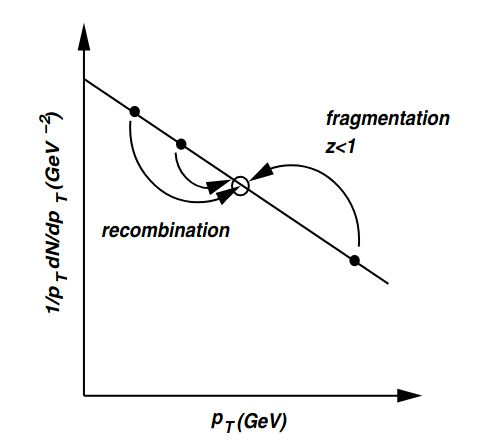
\includegraphics[width=0.5\linewidth]{res/fig/1-chapter/7-fragm-recom.jpg}
        \caption{Caption}
        \label{fig:7-fragm-recom}
    \end{figure}

\newpage

\section{Risultati sperimentali}

    \subsection{Adroni charmati in collisioni Pb-Pb a $\sqrt{s_{NN}} = \qty{5.02}{\tera \eV}$}

    \subsection{Adroni charmati in collisioni p-p a $\sqrt{s} = \qty{5.02}{\tera \eV}$ e a \\ $\sqrt{s} = \qty{13}{\tera \eV}$}